% Copyright 2004 by Till Tantau <tantau@users.sourceforge.net>.
%
% In principle, this file can be redistributed and/or modified under
% the terms of the GNU Public License, version 2.
%
% However, this file is supposed to be a template to be modified
% for your own needs. For this reason, if you use this file as a
% template and not specifically distribute it as part of a another
% package/program, I grant the extra permission to freely copy and
% modify this file as you see fit and even to delete this copyright
% notice. 

\documentclass{beamer}

\usepackage{blindtext}
\usepackage{tcolorbox}
\usepackage{soul}

\usefonttheme{professionalfonts} % using non standard fonts for beamer
\usefonttheme{serif} % default family is serif
%\usepackage{fontspec}
%\setmainfont{Liberation Serif}

% There are many different themes available for Beamer. A comprehensive
% list with examples is given here:
% http://deic.uab.es/~iblanes/beamer_gallery/index_by_theme.html
% You can uncomment the themes below if you would like to use a different
% one:
%\usetheme{AnnArbor}
%\usetheme{Antibes}
%\usetheme{Bergen}
%\usetheme{Berkeley}
%\usetheme{Berlin}
%\usetheme{Boadilla}
%\usetheme{boxes}
%\usetheme{CambridgeUS}
%\usetheme{Copenhagen}
%\usetheme{Darmstadt}
\usetheme{default}
%\usetheme{Frankfurt}
%\usetheme{Goettingen}
%\usetheme{Hannover}
%\usetheme{Ilmenau}
%\usetheme{JuanLesPins}
%\usetheme{Luebeck}
%\usetheme{Madrid}
%\usetheme{Malmoe}
%\usetheme{Marburg}
%\usetheme{Montpellier}
%\usetheme{PaloAlto}
%\usetheme{Pittsburgh}
%\usetheme{Rochester}
%\usetheme{Singapore}
%\usetheme{Szeged}
%\usetheme{Warsaw}



\title{Digital Signal Processing: Theory and Practice}

% A subtitle is optional and this may be deleted
\subtitle{\textbf{Sampling, quantization and number representation}}

\author{Sivakumar Balasubramanian}
% - Give the names in the same order as the appear in the paper.
% - Use the \inst{?} command only if the authors have different
%   affiliation.

\institute[Christian Medical College] % (optional, but mostly needed)
{
  \inst{}%
  Department of Bioengineering\\
  Christian Medical College, Bagayam\\
  Vellore 632002
}
% - Use the \inst command only if there are several affiliations.
% - Keep it simple, no one is interested in your street address.

\date{}
% - Either use conference name or its abbreviation.
% - Not really informative to the audience, more for people (including
%   yourself) who are reading the slides online

\subject{Lecture notes on signal processing}
% This is only inserted into the PDF information catalog. Can be left
% out.

% If you have a file called "university-logo-filename.xxx", where xxx
% is a graphic format that can be processed by latex or pdflatex,
% resp., then you can add a logo as follows:

% \pgfdeclareimage[height=0.5cm]{university-logo}{university-logo-filename}
% \logo{\pgfuseimage{university-logo}}

% Delete this, if you do not want the table of contents to pop up at
% the beginning of each subsection:
\AtBeginSubsection[]
{
  \begin{frame}<beamer>{Outline}
    \tableofcontents[currentsection,currentsubsection]
  \end{frame}
}

% Let's get started
\begin{document}

\begin{frame}
  \titlepage
\end{frame}

\begin{frame}{Sampling and interpolation}

\textbf{Sampling} is the process of converting a function $x(t)$ into a sequence $x[n]$.
\vspace{0.2in}

\textbf{Interpolation} is the process of converting a sequence $x[n]$ into a function $x(t)$.
\vspace{0.2in}

The following process is the foundation of digital signal processing,
	
\[ x(t) \longrightarrow x[n] \longrightarrow y[n] = H x[n] \longrightarrow y(t) \]

\end{frame}
%
%% DISCRETE SIGNALS AS VECTORS
%\begin{frame}{Discrete-time signals as vectors}
%
%Consider two finite duration real discrete-time signal 
%\[ x[n] = \{\boxed{x_0}, x_1\} = \left[x_0, x_1\right]^{T} \]
%\[ y[n] = \{\boxed{y_0}, y_1\} = \left[y_0, y_1\right]^{T} \]
%
%where, $n \in \{0, 1\}$
%
%\begin{figure}
%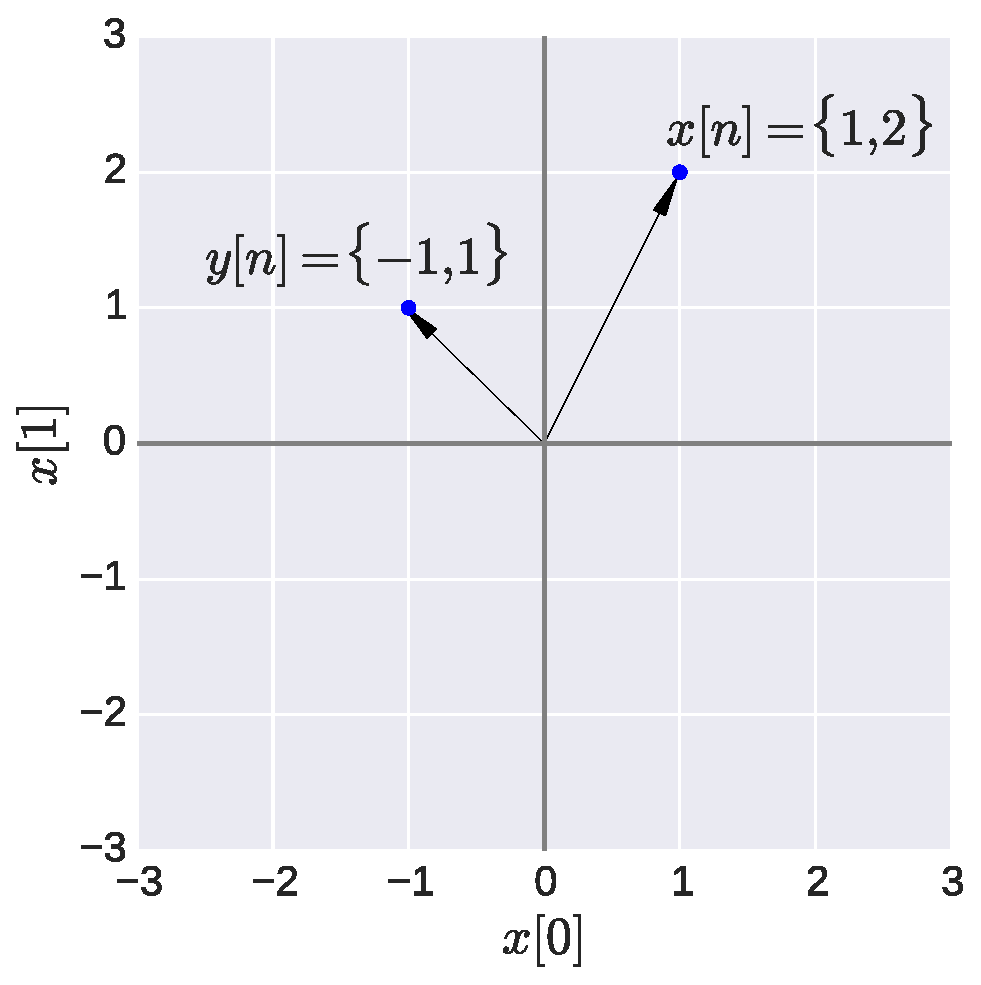
\includegraphics[width=0.5\textwidth]{img/2dvec.eps}
%\end{figure}
%\end{frame}
%
%% SOME FAMILIAR GEOMETRICAL IDEAS
%\begin{frame}{Some familiar and useful geometric ideas}
%
%\begin{itemize}
%\item \textbf{Length} of a vector.
%\[ \|x\| = \sqrt{x_0^2 + x_1^2} \]
%\item \textbf{Distance} between vectors.
%\[ \|x - y\| = \sqrt{\left(x_0 - y_0\right)^2 + \left(x_1 - y_1\right)^2} \]
%\item \textbf{Scalar product} or \textbf{Inner product} between vectors.
%\[ \langle x, y \rangle = x_0y_0 + x_1y_1 \implies \|x\| = \langle x, x \rangle \]
%\[ \langle x, y \rangle = \|x\| \|y\| \cos \theta \]
%\end{itemize}
%\end{frame}
%
%% Extension to N dimensions
%\begin{frame}{Extension to $N$ dimensions}
%Consider the following finite duration signals with $N$ elements,
%\[ x[n] = \{\boxed{x_0}, x_1, \cdots, x_{N-1}\} = \left[x_0, x_1, \cdots, x_{N-1}\right]^{T} \]
%\[ y[n] = \{\boxed{y_0}, y_1, \cdots, y_{N-1}\} = \left[y_0, y_1, \cdots, y_{N-1}\right]^{T} \]
%
%where, $x_i, y_i \in \mathbb{C}$
%
%\begin{itemize}
%\item \textbf{Length} of a vector. $\|x\| = \left(\sum_{i=0}^{N-1} \left|x_i\right| ^2\right)^{\frac{1}{2}}$
%\item \textbf{Distance} between vectors.$\|x - y\| = \left(\sum_{i=0}^{N-1} \left|x_i - y_i\right| ^2\right)^{\frac{1}{2}}$
%\item \textbf{Inner product} between vectors. $\langle x, y \rangle = \sum_{i=0}^{N-1}x_iy_i^*$
%\end{itemize}
%\end{frame}
%
%% EXTENSION TO INFINITE DIMENSIONS
%\begin{frame}{Extension to infinite dimensions!}
%
%Can we extend the geometric ideas to infinite dimensional signals?
%
%\textbf{Yes}, but we need to be careful.
%
%\[ x[n] = \{\boxed{x_0}, x_1, \cdots\} = \left[x_0, x_1, \cdots\right]^{T} \]
%\[ y[n] = \{\boxed{y_0}, y_1, \cdots\} = \left[y_0, y_1, \cdots\right]^{T} \]
%
%\begin{itemize}
%\item \textbf{Length} $\|x\| = \left(\sum_{i=0}^{\infty} \left|x_i\right| ^2\right)^{\frac{1}{2}}$
%\item \textbf{Distance} $\|x - y\| = \left(\sum_{i=0}^{\infty} \left|x_i - y_i\right| ^2\right)^{\frac{1}{2}}$
%\item \textbf{Inner product} $\langle x, y \rangle = \sum_{i=0}^{\infty}x_iy_i^*$
%\end{itemize}
%
%The above ideas make sense only when the infinite sums are finite converge, i.e. \textbf{the sums must converge}.
%
%\end{frame}
%
%% EXTENSION TO INFINITE DIMENSIONS
%\begin{frame}{Extension to infinite dimension!}
%
%We will restrict ourselves to the space of \textbf{finite energy signals}, i.e.
%\[ \|x\| = \left(\sum_{i \in \mathbb{Z}} \left|x_i\right| ^2\right)^{\frac{1}{2}} < \infty \]
%
%Here we have assumed $x[n]$ to start at $-\infty$ and end at $\infty$.
%
%\[ x[n] = \{\cdots, x_{-1}, \boxed{x_0}, x_1, \cdots\} = \left[\cdots, x_{-1}, x_0, x_1, \cdots\right]^{T} \]
%
%This also leads to meaningful inner products, 
%\[\|x\|, \|y\| < \infty \implies \left|\langle x, y\rangle\right| < \infty \]
%
%This is called the $\ell^2\left(\mathbb{Z}\right)$ space.
%
%\end{frame}
%
%% USE OF THE INNER PRODUCT
%\begin{frame}{What is the inner product?}
%\begin{itemize}
%\item Projection of a signal $x$ onto another signal $y$, or simply a measure of their relative orientations.
%
%\[ \langle x,y \rangle = \sum_{i \in \mathbb{Z}} x_iy_i^* = \|x\|\|y\|\cos \theta\]
%
%where, $\theta$ is the angle between the signals $x$ and $y$.
%
%\item $\langle x,y \rangle$ tells us how much of $x$ is in $y$ and \textit{vice versa}.
%\item $x$ and $y$ are orthogonal, when $\langle x,y \rangle = 0 \implies x \perp y$
%
%For example, let $x = \left[1, 1\right]^{T}$ and $y = \left[1, -1\right]^{T}$. What is  $\langle x,y  \rangle$ ?
%\end{itemize}
%\end{frame}
%
%% BASES 1
%\begin{frame}{\textbf{Bases}: Representing a signal in terms of other signals}\
%
%\begin{columns}
%	\begin{column}{.5\linewidth}
%	  Can $x[n]$ be represented as a linear combination of $x_0[n]$ and $x_1[n]$? \textbf{Yes.}
%	  
%	  \[ x[n] = \alpha_0x_0[n] + \alpha_1x_1[n] \]
%	  \[ \alpha_i = \frac{\langle x_i[n], x[n] \rangle}{\|x_i[n]\|}, i = 0, 1 \]
%	  
%	  \textbf{What are the values of $\alpha_1$ and $\alpha_2$?}
%
%	\end{column}
%	
%	\begin{column}{.5\linewidth}
%	\begin{figure}
%	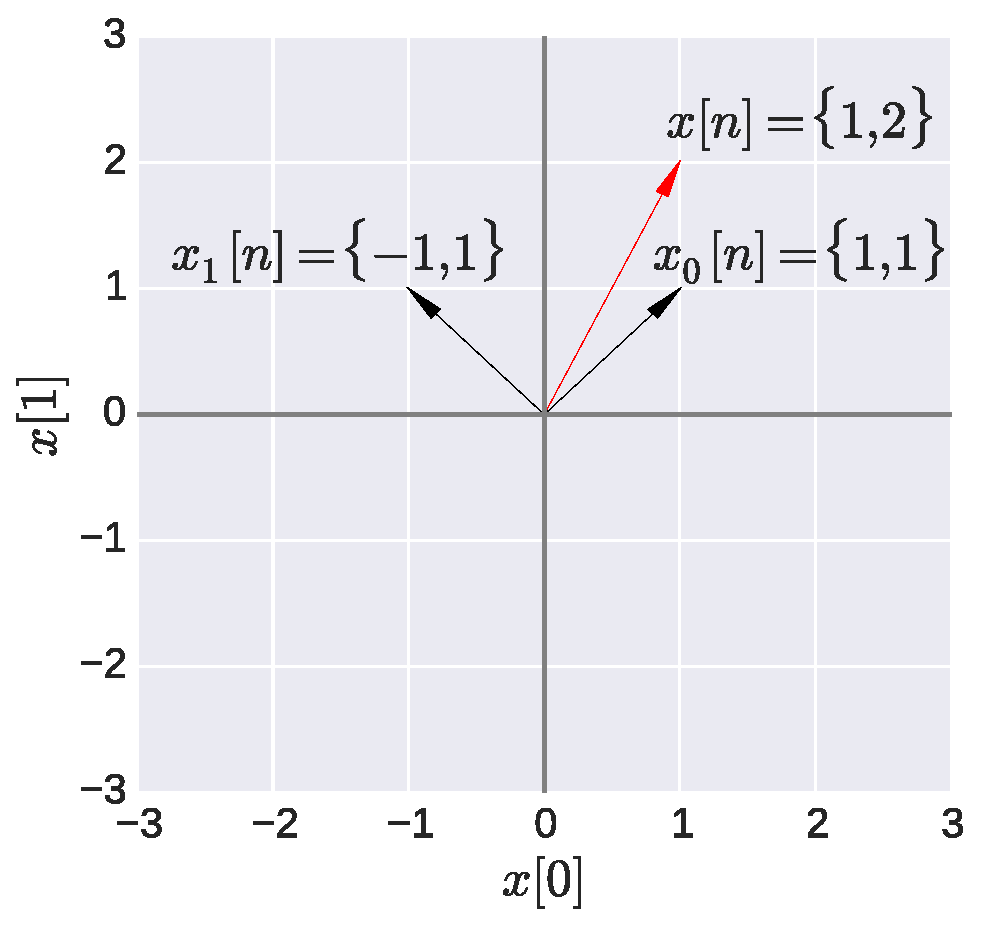
\includegraphics[width=\textwidth]{img/bases.eps}
%	\end{figure}
%	\end{column}
%\end{columns}
%\end{frame}
%
%% BASES 2
%\begin{frame}{\textbf{Bases}: Representing a signal in terms of other signals}\
%
%\begin{columns}
%	\begin{column}{.6\linewidth}
%		\begin{itemize}
%		\item $\{1,2\}$ and $\{\alpha_0, \alpha_1\}$ are two presentations of $x[n]$.
%		\item The difference is the basis.
%		\item Basis for $\{\alpha_0, \alpha_1\}$ is $\{x_0[n], x_1[n]\}$.
%		\item What is the basis for $\{1, 2\}$? $\implies$ the \textit{standard basis} $e_0 = \{1, 0\}$ and $e_1[n]=\{0,1\}$.
%		\end{itemize}
%	\end{column}
%	
%	\begin{column}{.4\linewidth}
%	\begin{figure}
%	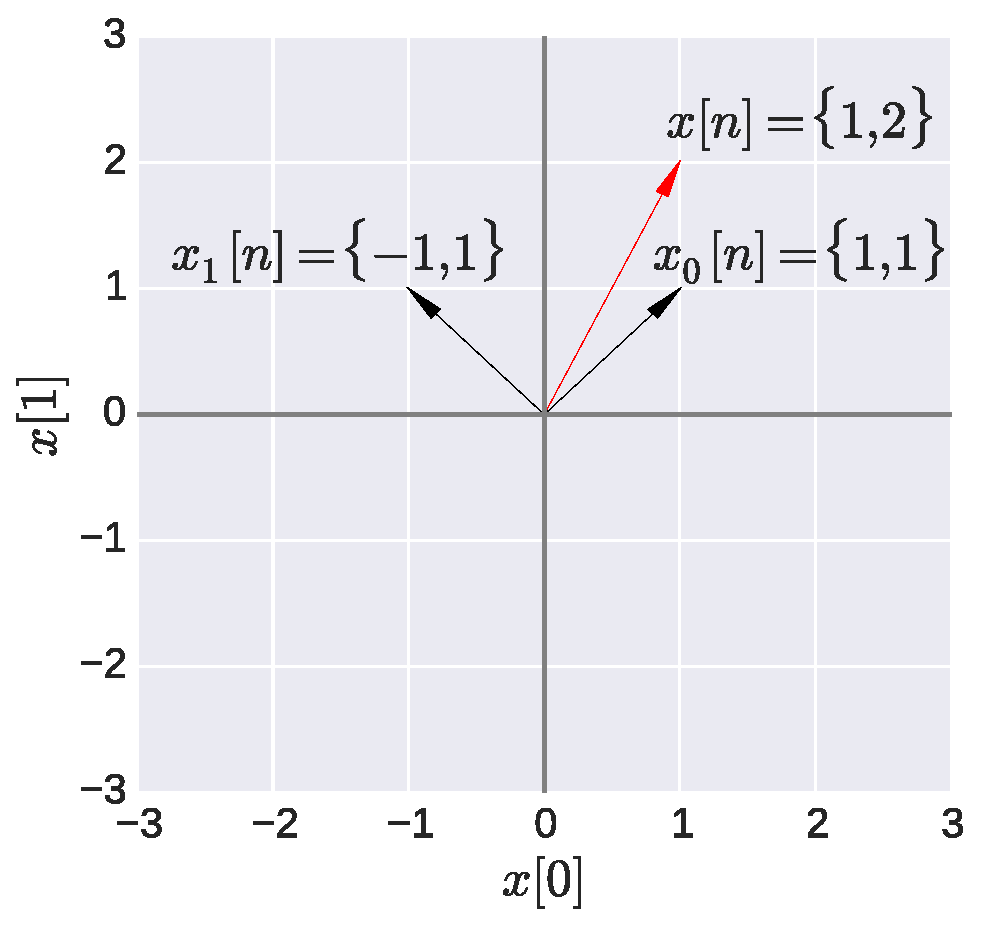
\includegraphics[width=\textwidth]{img/bases.eps}
%	\end{figure}
%	\end{column}
%\end{columns}
%\end{frame}
%
%% EXTENSION OF IDEAS TO CONTINUOUS-TIME
%\begin{frame}{Extension of ideas to continuous-time}
%
%Consider two continuous time signals, $x\left(t\right), y\left(t\right) \in \mathbb{C}^{\mathbb{R}}$, 
%\begin{itemize}
%\item \textbf{Length}.
%\[ \|x\| = \left(\int_{-\infty}^{\infty}{\left|x(t)\right|^2dt}\right)^{1/2} \]
%\item \textbf{Distance}.
%\[ \|x - y\| = \left(\int_{-\infty}^{\infty}{\left|x(t) - y(t)\right|^2dt}\right)^{1/2} \]
%\item \textbf{Scalar product} or \textbf{Inner product} between vectors.
%\[ \langle x, y \rangle = \left(\int_{-\infty}^{\infty}{x(t)y^*(t)dt}\right)^{1/2} \]
%\end{itemize}
%
%\textbf{Note:} The above quantities are meaningful only when the integrals converge.
%\end{frame}
%
%% EXTENSION OF IDEAS TO CONTINUOUS-TIME 2
%\begin{frame}{Extension to infinite dimension!}
%
%We will restrict ourselves to the space of \textbf{finite energy signals}, i.e.
%
%\[ \|x\| = \left(\int_{-\infty}^{\infty}{\left|x(t)\right|^2dt}\right)^{1/2} < \infty \]
%
%This is called the $\mathcal{L}^2\left(\mathbb{R}\right)$ space.
%
%\end{frame}

\end{document}


